%%%%%%%%%%%%%%%%%%%%%%%%%%%%%%%%%%%%%%%%%%%%%%%%%%%%%%%%%%%%%%%%%%%%%%
% How to use writeLaTeX:
%
% You edit the source code here on the left, and the preview on the
% right shows you the result within a few seconds.
%
% Bookmark this page and share the URL with your co-authors. They can
% edit at the same time!
%
% You can upload figures, bibliographies, custom classes and
% styles using the files menu.
%
% If you're new to LaTeX, the wikibook is a great place to start:
% http://en.wikibooks.org/wiki/LaTeX
%
%%%%%%%%%%%%%%%%%%%%%%%%%%%%%%%%%%%%%%%%%%%%%%%%%%%%%%%%%%%%%%%%%%%%%%
\documentclass{tufte-handout}

%\geometry{showframe}% for debugging purposes -- displays the margins

\usepackage{amsmath}
\usepackage{xcolor}
\usepackage{hyperref}
\usepackage{textcomp}

% Set up the images/graphics package
\usepackage{graphicx}
\setkeys{Gin}{width=\linewidth,totalheight=\textheight,keepaspectratio}
\graphicspath{{graphics/}}

\title{[Paper title] \newline Reproducibility Check Results}
\author{[Add reviewer name(s)] \\ dimeanalytics@worldbank.org}
\date{[Add date]}
% if the \date{} command is left out, the current date will be used

\usepackage{xcolor}

% The following package makes prettier tables.  We're all about the bling!
\usepackage{booktabs}
% The units package provides nice, non-stacked fractions and better spacing
% for units.
\usepackage{units}

% The fancyvrb package lets us customize the formatting of verbatim
% environments.  We use a slightly smaller font.
\usepackage{upquote}
\usepackage{fancyvrb}
\fvset{fontsize=\normalsize}
\renewcommand{\FancyVerbFormatLine}{\color{violet}}
\DefineShortVerb{\|}

% Small sections of multiple columns
\usepackage{multicol}

% Provides paragraphs of dummy text
\usepackage{lipsum}

% Packages and commands for the checkboxes
\usepackage{enumitem,amssymb}
\newlist{todolist}{itemize}{2}
\setlist[todolist]{label=$\square$}
\usepackage{pifont}
\newcommand{\cmark}{\ding{51}}%
\newcommand{\xmark}{\ding{55}}%
\newcommand{\done}{\rlap{$\square$}{\raisebox{2pt}{\large\hspace{1pt}\cmark}}%
\hspace{-2.5pt}}
\newcommand{\pending}{\rlap{$\square$}{\large\hspace{1pt}\xmark}}

% These commands are used to pretty-print LaTeX commands
\newcommand{\doccmd}[1]{\texttt{\textbackslash#1}}% command name -- adds backslash automatically
\newcommand{\docopt}[1]{\ensuremath{\langle}\textrm{\textit{#1}}\ensuremath{\rangle}}% optional command argument
\newcommand{\docarg}[1]{\textrm{\textit{#1}}}% (required) command argument
\newenvironment{docspec}{\begin{quote}\noindent}{\end{quote}}% command specification environment
\newcommand{\docenv}[1]{\textsf{#1}}% environment name
\newcommand{\docpkg}[1]{\texttt{#1}}% package name
\newcommand{\doccls}[1]{\texttt{#1}}% document class name
\newcommand{\docclsopt}[1]{\texttt{#1}}% document class option name

\newenvironment{nscenter}
 {\parskip=0pt\par\nopagebreak\centering}
 {\par\noindent\ignorespacesafterend}

\begin{document}

\maketitle% this prints the handout title, author, and date

\begin{marginfigure}%
  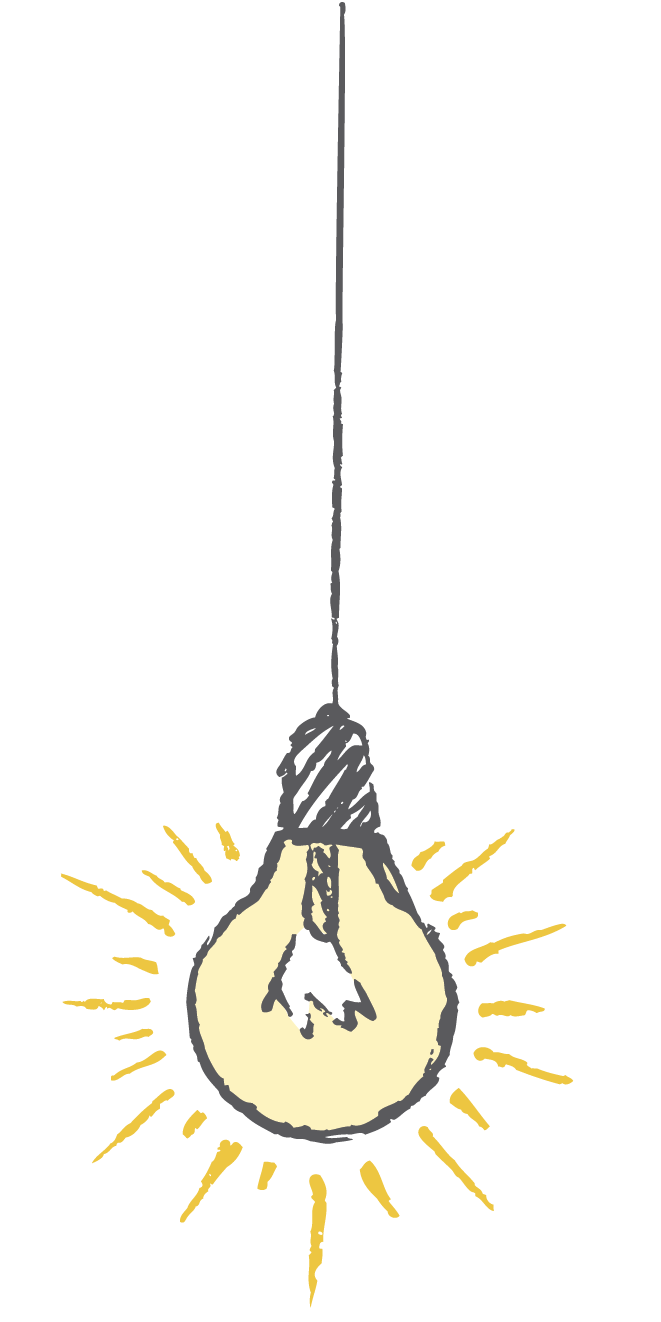
\includegraphics[width=\linewidth]{light.png}
\end{marginfigure}

%\printclassoptions
\section{Main findings}
\label{main-findings}

\begin{todolist}

    % replace \item with \item[\done] to add a check or with \item[\pending] to add an X

    \item[\done] The code ran in a new computer

    \item[\done] All the code outputs are stable over successive runs of the code

    \item[\done] All results that do not use restricted-access data were reproduced by the code
     
\end{todolist}

\section{System specifications}

Results were attempted to be reproduced in a computer with the following specifications:

\begin{itemize}
    \item OS: [add. Example:Windows 10 Enterprise, version 21H2]
    \item Processor: [add. Example: Intel(R) Core(TM) i7-8665U CPU @ 1.90GHz   2.11 GHz]
    \item Memory available: [add. Example: 15.8 GB]
    \item Software version: [add. Example: Stata 16.1]
\end{itemize}

\section{List of exhibits and reproducibility status}
\label{output-list}

% \textcolor{OliveGreen}{Reproduced}
% \textcolor{LimeGreen}{Results reproduced, but table or figure includes manual changes from code output}
% \textcolor{Gray}{Does not apply}
% \textcolor{Goldenrod}{All numbers reproduced, }
% \textcolor{BurntOrange}{Could not be verified: EXPLAIN WHY}
% \textcolor{Red}{Does not reproduce: EXPLAIN WHAT CHANGES. This includes cases when the outputs is either stable or unstable}

\textbf{Results in the Main Section of the Paper}

\noindent [List all exhibits in order of appearance in the paper]

\begin{itemize}

\item \textbf{Figure 1} \textcolor{OliveGreen}{[Add reproducibility status]}

\item \textbf{Table 1} \textcolor{OliveGreen}{[Add reproducibility status]}

...

\end{itemize}

\textbf{Results in the Appendix}

\noindent [List all exhibits in order of appearance in the appendix of the paper]

\begin{itemize}

\item \textbf{Appendix Table 1} \textcolor{OliveGreen}{[Add reproducibility status]}

\item \textbf{Appendix Figure 1} \textcolor{OliveGreen}{[Add reproducibility status]}

...

\end{itemize}

\end{document}